% Large-Scale Mapping in Drupal with the Geocluster-Leaflet Stack
% Author:       Eric Paul
% Organization: Phase2
%
% This text and presentation is released and licensed under GPL 3.0.
% You are free to reuse and distribute as you wish.
% @see http://opensource.org/licenses/GPL-3.0

\documentclass{beamer}

\usetheme{Warsaw}
\usepackage{color}
\usepackage{graphicx}
\usepackage{textpos}

\definecolor{p2orange}{RGB}{253,121,0}
\definecolor{p2dark}{RGB}{40,47,54}
\setbeamercolor{palette primary}{use=structure,fg=white,bg=p2orange}
\setbeamercolor{palette quaternary}{use=structure,fg=white,bg=p2dark}
\setbeamercolor{normal text}{use=structure,fg=p2dark}
\setbeamercolor{item}{fg=p2orange}

% For the lower-right corner logo.
\logo{
\includegraphics[scale=0.2]{assets/p2-logo-pinwheel.png}}

\begin{document}

% Meta for title slide.
\title[Large-Scale Mapping in Drupal with Geocluster \& Leaflet]{Scalable, Server-side Mapping in Drupal with the Geocluster-Leaflet Stack}  
\author[@mpgeek]{Eric Paul (@mpgeek)\\ \vspace{0.5em}
\includegraphics[scale=0.25]{assets/p2-logo_small.jpg}}
\institute {Phase2 Technology}
\date{DEV Lunch - \today} 

\begin{frame} 
  \maketitle
\end{frame}

\frame{\frametitle{Demo a Thing}
  \centerline{\href{http://vistacampus.gov/map}{http://vistacampus.gov/map}}
  \centerline{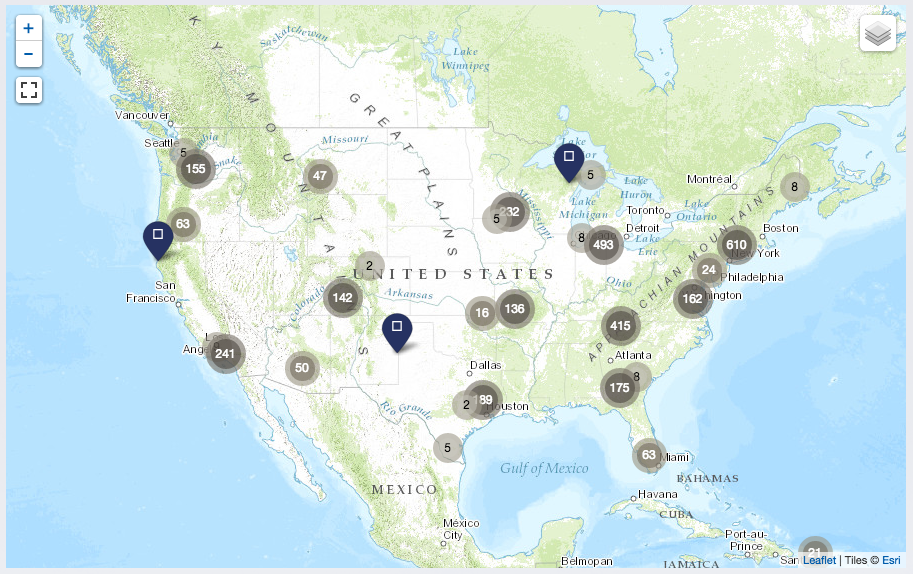
\includegraphics[scale=0.3]{assets/vista-map--static.png}}
}

\frame{\frametitle{The Recipe}
  \textbf{Basic Recipe}
  \begin{itemize}
    \item Address Field (location storage)
    \item Geocoder (geocoding addresses, requires GeoPHP)
    \item Geofield (geocode storage)
    \item \textbf{\textcolor{p2orange}{Geocluster}} (server-side clustering)
    \item Views
    \item Views GeoJSON (GeoJSON feeds)
    \item Leaflet GeoJSON (2.x for Panels support, 1.x for Bean)
    \item Leaflet Integration (requires Leaflet core library)
  \end{itemize}
  \vspace{1em}
  But... we need lots of \alert{patches}.
}

\frame{\frametitle{The Client Build}
  The client build was released as GPL2.0
  \begin{itemize}
    \item \href{https://github.com/mpgeek/Vista-Map}{https://github.com/mpgeek/Vista\-Map}
    \item \textcolor{lightgray}{Long and short-version slides + \LaTeX\  source is there as well}
  \end{itemize}
  \vspace{1em}
  Patch mania! How about a \textcolor{p2orange}{makefile}?
  \begin{itemize}
    \item \href{https://github.com/mpgeek/Vista-Map/blob/master/vista\_map.make}{https://github.com/mpgeek/Vista-Map/blob/master/vista\_map.make}
  \end{itemize}
}

\frame{\frametitle{Key Architectural Features}
  \textbf{Geocluster Keys}
  \begin{itemize}
    \item Clustering is performed at the \alert{query level} by Geocluster
    \item \textcolor{p2orange}{PHP} and \textcolor{blue}{JS} only see the clusters as single (Views) rows.
    \item This feature alone is almost \alert{entirely responsible} for the performance gain.
  \end{itemize}
  \pause
  \vspace{1em}
  But How?
  \begin{itemize}
    \item By \textcolor{p2orange}{geohashing}!
    \item See Wikipedia \href{http://en.wikipedia.org/wiki/Geohash}{Geohashing article} for more.\\ http://en.wikipedia.org/wiki/Geohash
  \end{itemize}
}

\frame{\frametitle{Geocluster \& Geohash}
  \textbf{In a nutshell:}
  \begin{itemize}
    \item Geocluster adds a hierarchical, spatial index to geofields based on the Geohash algorithm.
    \item Each geofield has columns for varying levels of precision (geohash index) created/updated on \textcolor{gray}{\texttt{entity\_save}}.
    \item A query for points/clusters specifies a geohash index and asks for clusters based on that index.
  \end{itemize}
  \pause
  \vspace{1em}
  \textbf{Notice:}
  \begin{itemize}
    \item The clustering information is created when the content is \alert{created/updated}.
    \item A request for points and clusters \alert{doesn't actually cluster}. Rather it's a \alert{simple query} of a spatial index. 
  \end{itemize}
}

\frame{\frametitle{Scalability Requirement}
  \textbf{How big did we need to go?}
  \vspace{0.5em}
  \begin{itemize}
    \item Mapping user profiles, about 18k users were migrated
    \vspace{0.5em}
    \item Originally, it was expected that all users would be mappped
    \vspace{0.5em}
    \item Application scale, then is $10\textsuperscript{4}$
  \end{itemize}
  \vspace{1em}
  \pause
  \textbf{Geocluster's clustering backend} is \alert{pluggable}, we get three out of the box:
  \vspace{1em}
  \begin{itemize}
  	\item PHP clustering (post-query clusternig)
	\vspace{0.5em}
	\item MySQL clustering (query-level clustering)
	\vspace{0.5em}
	\item Apache solr clustering (alternative query-level clustering)
  \end{itemize}
}

\frame{\frametitle{Scalability Metrics}
  \centerline{\textcolor{p2orange}{Cold caches}}
  \centerline{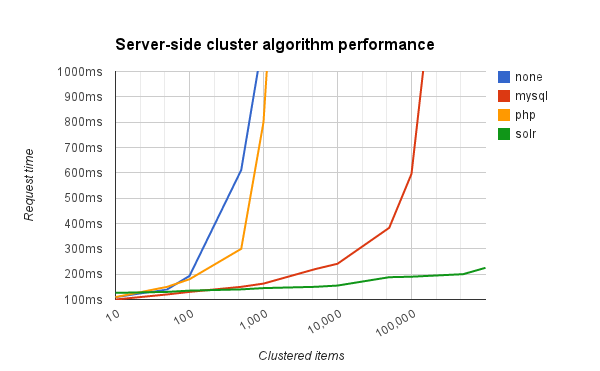
\includegraphics[scale=0.45]{assets/geocluster-performance.png}}
  \centerline{We implemented \alert{MySQL} clustering}
}

\frame{\frametitle{Possible Improvements}
  \textbf{Geocluster}
  \vspace{1em}
  \begin{itemize}
    \item \alert{Progressively enhance} with client side clustering below a certain point threshold. \href{https://www.drupal.org/node/1914704}{https://www.drupal.org/node/1914704}
    \vspace{0.5em}
    \item \textbf{Bounding works:} once zoomed in the cluster load is \alert{much smaller}
    \vspace{0.5em}
    \item The need for server-side clustering \textcolor{blue}{decreases} as zoom \textcolor{p2orange}{increases}
  \end{itemize}
}

\frame{\frametitle{Possible Improvements}
  \textbf{Leaflet GeoJSON}
  \begin{itemize}
    \item Collapse clusters to a single layer to eliminate layer interference.
    \vspace{0.5em}
    \pause
    \item Make data feeds cacheable by quantizing bounding box parameters.\\ \textcolor{gray}{\footnotesize{\texttt{/\$view\_url?bbox=\$left,\$right,\$top,\$bottom?zoom=\$zoom\_level}}}
    \vspace{0.5em}
    \begin{itemize}
      \item The \texttt{\textcolor{gray}{bbox}} arguments are floating-point numbers that depend on viewport size and zoom. \alert{Takes a long time for caches to warm up for non-mobile viewports}.
      \vspace{0.5em}
      \item \href{https://www.drupal.org/node/1868982}{https://www.drupal.org/node/1868982}
    \end{itemize}
  \end{itemize}
}

%\section{Takeaways}

%\frame{\frametitle{Take-out Knowledge}
%  \textbf{What we know}
%  \vspace{1em}
%  \begin{itemize}
%    \item Large-scale mapping is now possible in Drupal.
%    \vspace{0.5em}
%    \item Geocluster needs work.
%    \vspace{0.5em}
%    \item Leaflet GeoJSON needs work.
%    \vspace{0.5em}
%    \item Despite that, production-quality map applications can now be built.
%    \vspace{0.5em}
%    \pause
%    \item \alert{You will need a debugger}.
%  \end{itemize}
%}

\frame{\frametitle{References \& Resources}
  \textbf{Things we saw and more resources:}
  \begin{itemize}
  	\item Map application in production: \href{http://www.vistacampus.gov/map}{http://www.vistacampus.gov/map}
	\vspace{1em}
	\item Map application Drupal feature: \href{https://github.com/mpgeek/Vista-Map}{https://github.com/mpgeek/Vista-Map}
    \vspace{1em}
    \item Geohash Algorithm:\\ \href{http://en.wikipedia.org/wiki/Geohash}{http://en.wikipedia.org/wiki/Geohash}
    \vspace{1em}
    \item Geocluster Master's Thesis (by @dasjo): \href{http://dasjo.at/thesis}{http://dasjo.at/thesis}
  \end{itemize}
}


\end{document}